\documentclass[11pt,letterpaper,final]{report}
\usepackage[utf8]{inputenc}
\usepackage[english]{babel}
\usepackage{amsmath}
\usepackage{indentfirst}
\usepackage{amsfonts}
\addto{\captionsenglish}{\renewcommand{\bibname}{\LARGE{References}}}
\usepackage{pdfpages}
\usepackage{subcaption}
\usepackage{etoolbox}
\usepackage{amssymb}
\usepackage[font=small,labelfont=bf]{caption}
\usepackage{hanging}
\usepackage{notoccite}
\usepackage{float}
\usepackage{makeidx}
\usepackage{color}

\usepackage{multirow}


\usepackage{booktabs}% http://ctan.org/pkg/booktabs
\newcommand{\tabitem}{~~\llap{\textbullet}~~}


\usepackage{lscape}

\usepackage{enumitem}

\usepackage{titlesec}



\usepackage{gensymb}
\usepackage{hyperref}
\usepackage{graphicx}
\usepackage{lmodern}

\makeatletter
% section from book
%\newcommand\section{\@startsection {section}{1}{\z@}%
%                                   {-3.5ex \@plus -1ex \@minus -.2ex}%
%                                   {2.3ex \@plus.2ex}%
%                                   {\normalfont\Large\bfseries}}

\renewcommand\chapter{\@startsection {chapter}{0}{\z@}%
                                   {-1.5ex \@plus -1ex \@minus -.2ex}%
                                   {.5ex \@plus.2ex}% 
                                   {\normalfont\Large\textbf}}


\makeatletter

\renewcommand\section{\@startsection {section}{0}{\z@}%
                                   {-.1ex \@plus -1ex \@minus -.2ex}%
                                   {.05ex \@plus.2ex}% 
                                   {\normalfont\large\textbf}}


\makeatletter


\setlength{\parskip}{\baselineskip}%
\setlength{\parindent}{0pt}%






\usepackage{fourier}

\usepackage[left=1in,right=1in,top=1in,bottom=1in]{geometry}

\titleformat{\chapter}{\normalfont\huge}{\thechapter.}{20pt}{\huge\bf}
\titlespacing*{\chapter}{0pt}{-.5in}{20pt}
\author{Charles Hammond \\ Jaime Luo \\ Jacob Newman}


\begin{document}



\begin{center}

\begin{huge} 

\begin{Huge}\textbf{Work Plan} \end{Huge} \\~\\  UV System Replacement/UVT Requirement Reduction \\~\\
\end{huge}


\begin{Large} \textit{pHlux Engineering} \end{Large}



\begin{large}

\vspace{100pt}

\includegraphics[height=1.5in]{wp1}\\
\end{large}

\vspace{100pt}


\begin{tabular}{ll}
    \textbf{Prepared by:}&Charles Hammond\\
                         & Jaime Luo\\
                         & Jacob Newman\\
                         & \\~\\
    \textbf{Prepared for:}& Colleen Bronner\\
                         & \\~\\
    \textbf{Finalized on:}& \today\\ 

\end{tabular}

\end{center}

\pagenumbering{gobble}


\newpage
\setcounter{page}{0}


%%%%%%%%%%%%%%%%%%%%%%%%%%%%%%%%%%%%%%%%%%%%%%%%%%%%%%%%%%%%%
%%%%%%%%%%%%%%%%%%%%% Executive Summary %%%%%%%%%%%%%%%%%%%%%
%%%%%%%%%%%%%%%%%%%%%%%%%%%%%%%%%%%%%%%%%%%%%%%%%%%%%%%%%%%%%


\chapter*{Executive Summary}
\pagenumbering{roman} 

    \addcontentsline{toc}{chapter}{Executive Summary}

    This report contains the storm water management design requested by the city of Davis, California, on April 18th, 2018. The sources of stormwater are a tarmac, a grass-covered park, and a housing developement. The design includes a conveyance channel, gutters, inlets and a storm sewer for the housing development, a culvert, and a detention pond. The design is based on a 10-year storm.



    
    
\newpage
\setlength{\parskip}{0pt}%
\tableofcontents
\newpage
\listoffigures

\setlength{\parskip}{\baselineskip}%
\addcontentsline{toc}{chapter}{List of Figures}


\newpage
\chapter*{Nomenclature}
\addcontentsline{toc}{chapter}{Nomenclature}

\begin{table}[htbp]
\centering
\begin{tabular}{ccc}
\textbf{Symbol/Initialism} & \textbf{Meaning} & \textbf{Units} \\
\hline
NPDES & National Pollution Discharge Elimination System &  \\
UVT & Ultraviolet Transmissivity & \\
WWTP & Wastewater Treatment Plant & \\
CVRWQCB & Central Valley Regional Water Quality Control Board & \\
MPN & Most probable number &  \\
mgd & Million gallons per day & $10^6$ gal/day \\
ADP & Advanced Disinfection Process & \\
 kWh & kilowatt-hours % \\







\end{tabular} 
\end{table}


\newpage
\setcounter{chapter}{0}
\setcounter{figure}{0}
\setcounter{section}{0}

%%%%%%%%%%%%%%%%%%%%%%%%%%%%%%%%%%%%%%%%%%%%%%%%%%%%%%%%%%%%%%%%%%%%
%%%%%%%%%%%%%%%%%%%%% 1.0 Statement of Problem %%%%%%%%%%%%%%%%%%%%%
%%%%%%%%%%%%%%%%%%%%%%%%%%%%%%%%%%%%%%%%%%%%%%%%%%%%%%%%%%%%%%%%%%%%

\chapter{Statement of Problem}
\setcounter{page}{0}
\pagenumbering{arabic}
There are two problems that this project aims to solve for the UC Davis wastewater treatment plant (WWTP). First, the minimum UVT requirement of 55\% in the NPDES permit governing the plant results in yearly violations and fines. These violations are undesirable both financially, as the fines add up year after year, and legally, because willfully violating the law is not a viable or responsible solution. To resolve this, the UCD Utilities Division has requested a letter to the Water Board that justifies, based on data and rigorous testing, the reduction or removal of the UVT limit.

Second, the UV disinfection system is nearing the end of its planned service life and is in need of replacement. Because the WWTP discharges to Putah Creek, the Arboretum, and is even used for cooling buildings, the safety and compliance of the recycled water is of the utmost importance. An aging disinfection system could lead to water quality and reliability issues, which could lead to violations, fines, and perhaps even lawsuits. Thus, a replacement design has been requested by the UCD Utilities Division.




%%%%%%%%%%%%%%%%%%%%%%%%%%%%%%%%%%%%%%%%%%%%%%%%%%%%%%%%%%%%%%%%%%
%%%%%%%%%%%%%%%%%%%%% 2.0 Project Objectives %%%%%%%%%%%%%%%%%%%%%
%%%%%%%%%%%%%%%%%%%%%%%%%%%%%%%%%%%%%%%%%%%%%%%%%%%%%%%%%%%%%%%%%%

\setcounter{figure}{0}
\setcounter{section}{0} 
\chapter{Project Objectives}

There are two major objectives for this project:
\begin{enumerate}
\item Craft a memorandum intended for the Water Board that uses data from Carollo’s bioassay testing to justify the reduction or removal of the UVT requirement in the UC Davis WWTP’s NPDES permit.

\item Design a disinfection system that satisfies Title 22, fits within the current UV disinfection system footprint, utilizes the existing infrastructure, and minimizes energy consumption and cost.

\end{enumerate}

Success in completing these objectives will be measured by evaluating feedback from the client and by comparing actual vs. planned progress as detailed in the project timeline.



%%%%%%%%%%%%%%%%%%%%%%%%%%%%%%%%%%%%%%%%%%%%%%%%%%%%%%%%%%
%%%%%%%%%%%%%%%%%%%%% 3.0 Background %%%%%%%%%%%%%%%%%%%%%
%%%%%%%%%%%%%%%%%%%%%%%%%%%%%%%%%%%%%%%%%%%%%%%%%%%%%%%%%%

\setcounter{figure}{0}
\setcounter{section}{0}
\setcounter{table}{0}
\chapter{Background}

Wastewater treatment is usually divided into three main stages: primary, secondary, and tertiary. Primary treatment involves the removal of suspended solids and organic matter, secondary treatment typically includes the biological oxidation of organics remaining in the primary effluent, and tertiary treatment employs filters and/or disinfection processes to produce recycled water \cite{Metcalf}.
				 					
Disinfection is the process of destroying or inactivating pathogenic organisms, and considering the potential for human exposure to recycled wastewater, proper disinfection is extremely important. Of particular concern are bacteria, protozoan oocysts and cysts, viruses, and helminth ova, all of which can cause serious illness \cite{Metcalf}. Although many bacteria are harmless or beneficial, some present serious human health risks; for example, \textit{Legionella pneumophila} can cause malaise, myalgia, fever, headache, and respiratory illness \cite{Metcalf}.

Wastewater is usually disinfected with either chemical agents, such as chlorine or ozone, or non-ionizing radiation, most commonly ultraviolet light (UV) \cite{Metcalf}. Chlorine and ozone mainly function by oxidizing and destroying cell walls, while UV works mainly by damaging the RNA and DNA within a cell, rendering it incapable of reproducing \cite{Metcalf}. Combined UV-chemical treatments are known as UV-based advanced disinfection processes. For example, research has suggested that combining UV treatment with H$_2$O$_2$ could enhance viral deactivation \cite{Peizhe}. Each method has its strengths and weaknesses and each WWTP should tailor its disinfection process to its particular needs. For example, using chlorine or ozone can result in toxic disinfection byproducts (DPB), and while some viruses are resistant to UV irradiation, because UV disinfection works primarily by dimerizing adjacent thymine and cytosine DNA/RNA molecules, pathogens with thymine-rich genetic material (e.g., \textit{C. parvum} and Adenovirus) are more sensitive to UV disinfection \cite{Metcalf},\cite{ELShahawy2019}.

UV light is electromagnetic radiation with wavelengths between 100-400 nm, which is divided into longwave (UV-A), middlewave (UV-B), and shortwave (UV-C). The wavelength used for for disinfection is 254 nm and is generated by striking an electric arc between two electrodes in a lamp containing mercury\cite{ELShahawy2019}. UV lamps come in three general categories, 1) low-pressure, low-intensity (LPLI), 2) low-pressure, high-intensity (LPHI), and 3) medium-pressure, high intensity (MPHI) \cite{Metcalf}. Among the three types, LPLI and LPHI lamps are the most efficient, with 30-50\% and 35-50\% of their energy output in the form of monochromatic 254 nm wavelength light, respectively. MPHI lamps produce more intense light, but much less efficiently, with only 15-20\% of their energy output in the germicidal range \cite{Metcalf}.

The effectiveness of a given UV disinfection system depends on the chemical characteristics of the wastewater, presence of particulate matter, the target organisms, and the system design \cite{Metcalf}. These factors all influence the UV “dose”, which is defined as 



\setlength{\parskip}{0pt}
\begin{equation}
    D=I_{avg} \times t
  \end{equation}
  \begin{align*}
    \text{Where }&D= dose [mJ/cm^2]\\
    & I_{avg}= \text{average UV intensity }[mW/cm^2]\\
    & t=\text{exposure time,} s
  \end{align*}

  \setlength{\parskip}{\baselineskip}

Constituents in wastewater can influence the dose by reducing the average UV intensity. Typically these effects are measured via absorbance and transmittance, which is why the National Water Resources Institute (NWRI) recommends a general minimum of 55\% UV transmissivity for a UV dose of 100 $mJ/cm^2$ \cite{NPDES}. Dissolved iron and organic compounds with double bonds and aromatic functional groups are the most influential constituents, as they can directly absorb UV light \cite{Metcalf}. Particles can reduce disinfection performance by shielding harmful organisms from irradiation, reflecting and/or refracting light, and by harboring microorganisms \cite{Metcalf}.

Contact basins can be either open channels or closed reactors and, due to the relatively short contact time, they must be carefully designed to ensure complete disinfection \cite{Metcalf}. Hydraulic design of a UV disinfection system is extremely important, as non-ideal hydraulics can lead to longitudinal mixing, which leads to a distributed, rather than uniform, exposure time \cite{Metcalf}. Two important challenges when designing a UV disinfection system are ensuring uniform velocity fields approaching and exiting the UV banks, and ensuring equal flow between channels; both issues could result in over or underdosing \cite{Metcalf}. Optimization models have suggested that dose distributions and flow characteristics for open-channel reactors are most dependent on the lamp configuration \cite{Sultan2019}. Alternatively, closed vessel UV reactors offer several advantages, including improved hydraulics, reduced construction costs, and lower power requirements \cite{Evoqua}. 

The required dose is most commonly determined via a collimated beam bioassay in which a known UV dose is applied to a small batch reactor and correlated to the organism inactivation results, which is typically reported in most probable number (MPN) and must fall between quality-control limits set by the EPA \cite{Metcalf}. Organisms used for determining the required dose include Bacteriophage MS2 and \textit{B. subtilus} \cite{Metcalf}.

\section{Site History}

The current UCD WWTP replaced its 52 year old predecessor 1999 for \$15.3 million, serves over 21,000 students and 9,500 faculty, and is rated for 2.8 million gallons per day (mgd), though it usually operates at around 1.6 mgd \cite{Kerlin}, \cite{Facilities}. It discharges recycled water to the south fork of Putah Creek and the UCD Arboretum in addition to providing recycled water (as defined in Title 22) to the UCD Central Heating and Cooling Plant \cite{NPDES}, \cite{DaveJones}. The plant underwent an expansion in 2007 that resulted in the addition of a third UV disinfection channel. Additionally, the wastewater source profile is challenging, as UC Davis has many animal teaching facilities that produce low-transmittance runoff, especially during large rainfall events.

\section{Regulations} 

The 1969 Porter-Cologne Water Quality Control Act is provides the legal framework for water recycling in California, and Title 22 requires the Department of Health Services to set water and bacteriological treatment standards \cite{WEF}. The CRWQCB, which is one of nine regional boards, sets standards with help from the Department of Public Health and issues individual discharge permits, known as NPDES permits \cite{WEF}. Recycled water can be used for irrigation, landscaping, air conditioning, commercial laundry, decorative fountains, and toilets in commercial buildings \cite{WEF}. The 55\% UVT standard in the UCD WWTP’s NPDES permit is from the National Water Resources Institute (NWRI) and is mandated by Title 22 \cite{NPDES}.

    
 
\section{Precedents}

Trojan UV, whose technology the current UV disinfection system utilizes, claims that UV treatment can be used on wastewater with a transmittance as low as 15\% and provides a case study where effective disinfection was achieved in a 54.3 mgd combined wastewater and stormwater treatment plant with as low as 30\% UVT using the TrojanUV4000Plus \cite{TrojanUV1}. They claim the key to effective disinfection is to optimize the “effective water layer” by manipulating the reactor hydraulics and lamp output and spacing \cite{TrojanLowUVT}.

  


%%%%%%%%%%%%%%%%%%%%%%%%%%%%%%%%%%%%%%%%%%%%%%%%%%%%%%%%%%%%%%%%%%%%
%%%%%%%%%%%%%%%%%%%%% 4.0 Technical Approach %%%%%%%%%%%%%%%%%%%%%%%
%%%%%%%%%%%%%%%%%%%%%%%%%%%%%%%%%%%%%%%%%%%%%%%%%%%%%%%%%%%%%%%%%%%%

\setcounter{figure}{0}
\setcounter{section}{0}
\setcounter{table}{0}
\chapter{Technical Approach}

pHlux Engineering’s approach to this project is based on a thorough study of the principles of UV disinfection and an analysis of historical and present plant operations data. After analyzing and interpreting the data from a bioassay test of the existing UV system, the engineering team will draft and finalize a memorandum to the California Regional Water Quality Control Board (CRWQCB) with recommendations on modifying the UVT requirement in the discharge permit. For the design of the new disinfection system, UV will be compared to chlorine and ozone to determine the cheapest and safest alternative. The engineering team will then develop multiple designs utilizing  the chosen disinfection method and evaluate their performance based on criteria such as cost, energy efficiency, and use of existing infrastructure. Once a final design has been agreed upon and optimized, work will begin on preparing the final design deliverables. A full list of project tasks is presented below.

\begin{enumerate}[topsep=0pt,itemsep=-0ex,partopsep=0ex,parsep=0ex]
    \item Literature review
    \begin{enumerate}[topsep=0pt,itemsep=-0ex,partopsep=0ex,parsep=0ex]
            \item Review UV disinfection concepts and best practices
            \item Review permits and regulations
    \end{enumerate}
    \item Client meeting and site assessment
    \item Data collection
    \begin{enumerate}[topsep=0pt,itemsep=-0ex,partopsep=0ex,parsep=0ex]
        \item  Bioassay test
        \item Historical data
    \end{enumerate}
    \item Data analysis and interpretation
    \item Author memorandum
    \item Disinfection method alternatives analysis
    \item Preliminary design and alternatives development
    \begin{enumerate}[topsep=0pt,itemsep=-0ex,partopsep=0ex,parsep=0ex]
        \item UV dosage
        \item Fouling prevention mechanisms
        \item Lamp specifications
    \end{enumerate}
    \item Alternatives analysis
    \item Preparation of final design deliverables
\end{enumerate}

\section{Literature Review}

To begin this project, the engineering team performed a literature review of UV disinfection principles to identify relevant design parameters and best management practices for UV disinfection. Operational hazards associated with UV radiation were studied to understand how best to mitigate risks in the final design. The preliminary research phase also included a review of all regulations and permits that influence the design and operation of the WWTP. Special attention was given to  Title 22 standards for tertiary treated recycled water and the UCD WWTP’s  unique NPDES permit. Additionally, pHlux Engineering plans to analyze case-studies concerning UV performance under low UVT conditions to provide better informed recommendations regarding the plant’s UVT exceedances. 

\section{Client Meeting and Site Assessment}

The project team met with Courtney Hall from the UC Davis Utilities Division (Utilities Division) to discuss the client’s needs and desires. During the meeting Ms. Hall informed the engineering team that UV disinfection was originally chosen for the UCD WWTP at the recommendation of UC Davis environmental engineering faculty. She also expressed the Utilities Division’s desire to replace the existing UV system with another UV project because of the staff’s familiarity with this disinfection method. This meeting was followed by a visit to the WWTP to document the existing UV disinfection system and to observe a bioassay test performed by Carollo Engineers.

\section{Data Collection}

The UC Davis Utilities Division provided historical data for the daily plant and UV channel flows as well as bacterial test data for the performance of the existing disinfection system. The Utilities Division also supplied PDFs of the as-built construction drawings for the WWTP that will be used to assess the existing footprint of the UV disinfection system. Additionally, the Utilities Division will provide the results from Carollo Engineers’ bioassay test as well as historical data for the UVT of the UV system influent. Rainfall data for the UC Davis campus will be taken from the historical record of the UC Davis Department of Atmospheric Science, which operates an on-campus weather station. 

\section{Data Analysis and Interpretation}

The historical rainfall and UVT data will be used to compute the average rainfall event size that causes a UVT exceedance and how frequently these violations occur. Next, the results of the bioassay test will be analyzed to determine the minimum allowable UVT at which the existing UV system is able to meet its NPDES disinfection requirement. Recommendations will be made to revise the existing NPDES permit based on the determined frequency of UVT exceedance and the minimum allowable UVT.
 
The historical flow and bacterial test data will be used by the engineering team to properly size the new disinfection system and to determine the required disinfection dose. Additionally, these two sets of data will be used to run and verify  a  model that pHlux Engineering will create to assess the alternative disinfection system designs.

NEEDS REST OF SECTIONS 4.5 to end


%%%%%%%%%%%%%%%%%%%%%%%%%%%%%%%%%%%%%%%%%%%%%%%%%%%%%%%%%%%%
%%%%%%%%%%%%%%%%%%%%% 5.0 Deliverables %%%%%%%%%%%%%%%%%%%%%
%%%%%%%%%%%%%%%%%%%%%%%%%%%%%%%%%%%%%%%%%%%%%%%%%%%%%%%%%%%%


\setcounter{figure}{0}
\setcounter{section}{0}
\setcounter{equation}{0}
\setcounter{table}{0}
\chapter{Deliverables}

For this project, pHlux Engineering is tasked with completing multiple deliverables for the client. The first main deliverable will be a technical memorandum that uses data from a bioassay test conducted at the UCD WWTP by Carollo Engineers to make recommendations to the Central Valley Regional Water Board to modify the current UVT limits set by the NPDES permit. The final draft of this memorandum will be completed and submitted by April 5, 2019. 

The second deliverable will be the final design of a new UV disinfection system. This will be a deliverable that will not be directly submitted to the client, but will be presented in the final deliverables. pHlux Engineering will have this final design completed by May 19, 2019 so that there is adequate time to complete the final deliverables. The final deliverables consist of a poster to be presented at the Senior Design Showcase on June 6, 2019, a final presentation to the client on May 19, 2019, a media release video to be submitted by June 7, 2019, and a final report due on June 13, 2019. These final deliverables will summarize the entire design process, from defining the problem to considering alternative solutions to selecting the final design based on cost, efficiency, and environmental considerations 




%%%%%%%%%%%%%%%%%%%%%%%%%%%%%%%%%%%%%%%%%%%%%%%%%%%%%%%%%%%%%%%%%%
%%%%%%%%%%%%%%%%%%%%% 6.0 Project Management %%%%%%%%%%%%%%%%%%%%%
%%%%%%%%%%%%%%%%%%%%%%%%%%%%%%%%%%%%%%%%%%%%%%%%%%%%%%%%%%%%%%%%%%



\setcounter{figure}{0}
\setcounter{section}{0}
\setcounter{table}{0}
\chapter{Project Management}

The pHlux Engineering team consists of Charles Hammond, Jaime Luo, and Jacob Newman. Charles is the Programming Specialist and Scribe for this project, and will be responsible for documenting meetings. He has environmental engineering experience with the Los Angeles County Sanitation Districts (LACSD) and is experienced with  the software programs that will be used in this project, including AutoCAD, FlowMaster, and MATLAB. Jaime is the Facilitator and Time Manager for this project and will be responsible for ensuring the team meets deadlines and updating the project timeline as necessary. She has taken water and environmental engineering courses at UC Davis and has experience working with Flowmaster and AutoCAD. As the Project Liaison and Editor, Jacob is in charge of all communication with the client and advisors and will serve as the final editor on all written documents. His qualifications include relevant water treatment and design courses and prior experience working with LACSD, including extensive experience working with project managers and equipment vendors. 

This project will require knowledge of wastewater systems and the regulations related to UV disinfection.. In addition to technical knowledge,  this project will require knowledge of project management to design a new UV disinfection system that fits the client’s needs and stays within the project constraints. This project will require strong writing skills for the technical memorandum and final report. The pHlux Engineering team is highly adept and well-rounded in both technical engineering and writing, and will apply these skills to produce high-quality results.

Given that this project will require many intermediary steps to achieve the final design, time management will be crucial for efficiently completing the project. To help organize the project timeline and manage tasks and deadlines, a Gantt Chart detailing major tasks and milestones will be used. This Gantt Chart, shown below in Figure 1, will assist the engineers with tracking the progress of the project and keeping them on schedule. The chart is divided into two sections for the two project objectives--the UVT memorandum and the UV disinfection system design. Each section is divided into subsections to provide more detail.


%%%%%%%%%%%%%%%%%%%%%%%%%%%%%%%%%%%%%%%%%%%%%%%%%%%%%%%%%%%%%%%
%%%%%%%%%%%%%%%%%%%%% 7.0 Risk Management %%%%%%%%%%%%%%%%%%%%%
%%%%%%%%%%%%%%%%%%%%%%%%%%%%%%%%%%%%%%%%%%%%%%%%%%%%%%%%%%%%%%%

\setcounter{figure}{0}
\setcounter{section}{0}
\setcounter{table}{0}
\chapter{Risk Management}

As with any engineering project, there are risks associated that can affect the course of the project and the performance of the team. The potential risks for this project and prevention/mitigation strategies are summarized in Table X below. For controllable risks, preventative measures can be taken and for uncontrollable risks, mitigative measures can be taken.

\begin{table}[H]
    \centering
    \caption{Risk management.}

    \def\arraystretch{1}
    \begin{tabular}{c|ll}

\textbf{}&\textbf{Risk}&\textbf{Prevention/Mitigation} \\ \hline


\multirow{7}{*}{Controllable} & Safety during WWTP visits &  Inform facility of visit \\
   &  &  Bring a partner \\
   &  &  Wear PPE \\ [.3\normalbaselineskip]  %use \tabitem to put a bullet
   &  Software trouble &  Use peer resources through Slack \\[.3\normalbaselineskip]
    &  Overambitious goals &  Consider alternatives \\[.3\normalbaselineskip]
   &  Writing in one voice &  Collaborate and familiarize writing styles \\[.3\normalbaselineskip]
   & Team Conflicts &  Communicate openly and reach out to advisors if necessary \\[.3\normalbaselineskip] \hline
   \multirow{3}{*}{Uncontrollable} & Illness/emergencies &  Be flexible\\
   &  &  Redistribute tasks\\
    &  &  Communicate with client about changes \\
\end{tabular} 
\end{table}


These risks are all very possible and realistic for this project, however, pHlux Engineering will be applying the preventative strategies throughout their engineering process to reduce the probability of the controllable risks occurring. The chances of the uncontrollable risks occurring is unpredictable, but in the chance that an unforeseen circumstance does arise, the team will be proactive and flexible in adjusting their engineering process and the project scope to manage the impacts that would arise. 


% \begin{figure}[H]
%     \centering
%     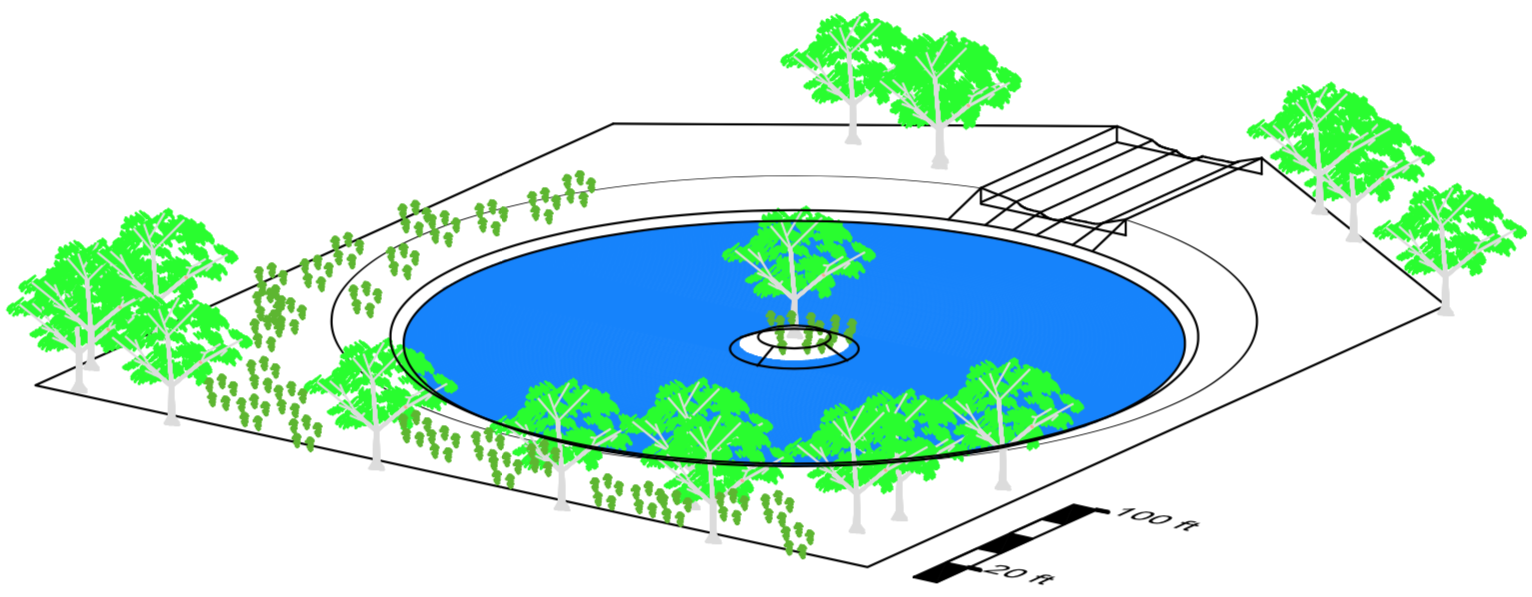
\includegraphics[height=.2\textheight]{F3P.png}
%     \caption{Impression of what the pond may look like after landscaping. }
% \end{figure}

%%%%%%%%%%%%%%%%%%%%%%%%%%%%%%%%%%%%%%%%%%%%%%%%%%%%%%%%%%%%%%%%%%
%%%%%%%%%%%%%%%%%%%%% 8.0 Required Resources %%%%%%%%%%%%%%%%%%%%%
%%%%%%%%%%%%%%%%%%%%%%%%%%%%%%%%%%%%%%%%%%%%%%%%%%%%%%%%%%%%%%%%%%

\setcounter{figure}{0}
\setcounter{section}{0}
\setcounter{table}{0}
\chapter{Required Resources}


For this project, an estimated 15 person hours/week is expected from each engineer, totalling a cumulative 675 hours over the course of 15 weeks. This includes approximately 9 individual person hours/week spent in lectures, labs, and meetings. The remaining 6 person hours per week will be spent on the major tasks over the estimated time it will take to complete as detailed in the Gantt Chart, with some of the major tasks overlapping. A breakdown of these person hours are shown in Table X in the Appendix. The engineers recognize that these hours are estimates and will fluctuate over the course of the projects and will be flexible to adjust as needed to meet deadlines. 

pHlux Engineering will will request access from the client to conduct site visits to the UCD Wastewater Treatment Plant to understand the project site better and to document the current system’s features. The drafting of the technical memorandum and the design of a UV disinfection system will require the use of various resources. For the technical memorandum, data from a bioassay test conducted by Carollo Engineers and historical rainfall data, provided by Carollo Engineers and the client, will be used. To design a new UV disinfection system, the historical rainfall data, most probable number data, and existing system as-builts will be requested from the client to create a new system. Various software programs, including AutoCAD, FlowMaster, and Matlab, will be used to analyze the data and model the design.

NEEDS TABLE


%%%%%%%%%%%%%%%%%%%%%%%%%%%%%%%%%%%%%%%%%%%%%%%%%%%%%%%%%%%
%%%%%%%%%%%%%%%%%%%%% 10.0 Appendix A %%%%%%%%%%%%%%%%%%%%%
%%%%%%%%%%%%%%%%%%%%%%%%%%%%%%%%%%%%%%%%%%%%%%%%%%%%%%%%%%%
\newpage
\setcounter{figure}{0}
\setcounter{section}{0}
\setcounter{table}{0}
\chapter*{Appendix A - Resumes}
\addcontentsline{toc}{chapter}{Appendix A - Resumes}

\renewcommand{\thefigure}{A.\arabic{figure}}
\setcounter{figure}{0}

\begin{landscape}
\newpage
\setcounter{figure}{0}
\setcounter{section}{0}
\setcounter{table}{0}
\chapter*{Appendix B - Assessment Criteria}
\addcontentsline{toc}{chapter}{Appendix B - Assessment Criteria}
\renewcommand{\thefigure}{B.\arabic{figure}}
\setcounter{figure}{0}

\begin{table}[H]
    \centering
    \caption{Assessment criteria for alternatives.}

    \def\arraystretch{2}
    \begin{tabular}{lccc}

\textbf{Criteria}&\textbf{Assessment Tool}&\textbf{Performance Metric}&\textbf{Threshold for Success} \\ \hline

Capital Cost & Literature/manufacturer Estimates & Dollars to Construct & Lowest \\
O\&M Cost & Literature/manufacturer Estimates & Annual Cost of O\&M & Lowest \\
Maintenance Requirements & Literature/manufacturer Estimates & Weekly person-hours & Lowest \\
Operational Hazards & Literature/manufacturer Information & Number of safety concerns & Fewest \\
Meets Title 22 standards & Title 22 & $\frac{\text{Standards met}}{\text{\# of standards}}$& 100\% \\
Utilizes Existing Infrastructure & Inventory of existing onsite infrastructure & Dollars saved by using existing equipment & Greatest savings \\
Energy Efficiency & Literature and manufacturer’s specifications & $\frac{\text{kWh input}}{\text{kWh output}}$ & Closest to 1 \\
Life Cycle Assessment & Literature/manufacturer Estimates & Annual Cost of O\&M & Lowest \\
Permissible UVT & Literature/manufacturer Estimates & UVT (\%) & Less than 55\% \\
System Lifetime & Literature/manufacturer Estimates & Years & $\geq 20$ \\ \hline


\end{tabular} 
\end{table}
\end{landscape}





\begin{flushleft}
\newpage
\bibliography{bib} 
\bibliographystyle{ieeetr} 
\end{flushleft}

\end{document}
